
%% bare_jrnl.tex
%% V1.4b
%% 2015/08/26
%% by Michael Shell
%% see http://www.michaelshell.org/
%% for current contact information.
%%
%% This is a skeleton file demonstrating the use of IEEEtran.cls
%% (requires IEEEtran.cls version 1.8b or later) with an IEEE
%% journal paper.
%%
%% Support sites:
%% http://www.michaelshell.org/tex/ieeetran/
%% http://www.ctan.org/pkg/ieeetran
%% and
%% http://www.ieee.org/

%%*************************************************************************
%% Legal Notice:
%% This code is offered as-is without any warranty either expressed or
%% implied; without even the implied warranty of MERCHANTABILITY or
%% FITNESS FOR A PARTICULAR PURPOSE! 
%% User assumes all risk.
%% In no event shall the IEEE or any contributor to this code be liable for
%% any damages or losses, including, but not limited to, incidental,
%% consequential, or any other damages, resulting from the use or misuse
%% of any information contained here.
%%
%% All comments are the opinions of their respective authors and are not
%% necessarily endorsed by the IEEE.
%%
%% This work is distributed under the LaTeX Project Public License (LPPL)
%% ( http://www.latex-project.org/ ) version 1.3, and may be freely used,
%% distributed and modified. A copy of the LPPL, version 1.3, is included
%% in the base LaTeX documentation of all distributions of LaTeX released
%% 2003/12/01 or later.
%% Retain all contribution notices and credits.
%% ** Modified files should be clearly indicated as such, including  **
%% ** renaming them and changing author support contact information. **
%%*************************************************************************


% *** Authors should verify (and, if needed, correct) their LaTeX system  ***
% *** with the testflow diagnostic prior to trusting their LaTeX platform ***
% *** with production work. The IEEE's font choices and paper sizes can   ***
% *** trigger bugs that do not appear when using other class files.       ***                          ***
% The testflow support page is at:
% http://www.michaelshell.org/tex/testflow/



\documentclass[journal]{IEEEtran}
%
% If IEEEtran.cls has not been installed into the LaTeX system files,
% manually specify the path to it like:
% \documentclass[journal]{../sty/IEEEtran}





% Some very useful LaTeX packages include:
% (uncomment the ones you want to load)


% *** MISC UTILITY PACKAGES ***
%
%\usepackage{ifpdf}
% Heiko Oberdiek's ifpdf.sty is very useful if you need conditional
% compilation based on whether the output is pdf or dvi.
% usage:
% \ifpdf
%   % pdf code
% \else
%   % dvi code
% \fi
% The latest version of ifpdf.sty can be obtained from:
% http://www.ctan.org/pkg/ifpdf
% Also, note that IEEEtran.cls V1.7 and later provides a builtin
% \ifCLASSINFOpdf conditional that works the same way.
% When switching from latex to pdflatex and vice-versa, the compiler may
% have to be run twice to clear warning/error messages.






% *** CITATION PACKAGES ***
%
%\usepackage{cite}
% cite.sty was written by Donald Arseneau
% V1.6 and later of IEEEtran pre-defines the format of the cite.sty package
% \cite{} output to follow that of the IEEE. Loading the cite package will
% result in citation numbers being automatically sorted and properly
% "compressed/ranged". e.g., [1], [9], [2], [7], [5], [6] without using
% cite.sty will become [1], [2], [5]--[7], [9] using cite.sty. cite.sty's
% \cite will automatically add leading space, if needed. Use cite.sty's
% noadjust option (cite.sty V3.8 and later) if you want to turn this off
% such as if a citation ever needs to be enclosed in parenthesis.
% cite.sty is already installed on most LaTeX systems. Be sure and use
% version 5.0 (2009-03-20) and later if using hyperref.sty.
% The latest version can be obtained at:
% http://www.ctan.org/pkg/cite
% The documentation is contained in the cite.sty file itself.






% *** GRAPHICS RELATED PACKAGES ***
%
\ifCLASSINFOpdf
  \usepackage[pdftex]{graphicx}
  % declare the path(s) where your graphic files are
  % \graphicspath{{../pdf/}{../jpeg/}}
  % and their extensions so you won't have to specify these with
  % every instance of \includegraphics
  % \DeclareGraphicsExtensions{.pdf,.jpeg,.png}
\else
  % or other class option (dvipsone, dvipdf, if not using dvips). graphicx
  % will default to the driver specified in the system graphics.cfg if no
  % driver is specified.
  \usepackage[dvips]{graphicx}
  % declare the path(s) where your graphic files are
  % \graphicspath{{../eps/}}
  % and their extensions so you won't have to specify these with
  % every instance of \includegraphics
  % \DeclareGraphicsExtensions{.eps}
\fi
% graphicx was written by David Carlisle and Sebastian Rahtz. It is
% required if you want graphics, photos, etc. graphicx.sty is already
% installed on most LaTeX systems. The latest version and documentation
% can be obtained at: 
% http://www.ctan.org/pkg/graphicx
% Another good source of documentation is "Using Imported Graphics in
% LaTeX2e" by Keith Reckdahl which can be found at:
% http://www.ctan.org/pkg/epslatex
%
% latex, and pdflatex in dvi mode, support graphics in encapsulated
% postscript (.eps) format. pdflatex in pdf mode supports graphics
% in .pdf, .jpeg, .png and .mps (metapost) formats. Users should ensure
% that all non-photo figures use a vector format (.eps, .pdf, .mps) and
% not a bitmapped formats (.jpeg, .png). The IEEE frowns on bitmapped formats
% which can result in "jaggedy"/blurry rendering of lines and letters as
% well as large increases in file sizes.
%
% You can find documentation about the pdfTeX application at:
% http://www.tug.org/applications/pdftex





% *** MATH PACKAGES ***
%
%\usepackage{amsmath}
% A popular package from the American Mathematical Society that provides
% many useful and powerful commands for dealing with mathematics.
%
% Note that the amsmath package sets \interdisplaylinepenalty to 10000
% thus preventing page breaks from occurring within multiline equations. Use:
%\interdisplaylinepenalty=2500
% after loading amsmath to restore such page breaks as IEEEtran.cls normally
% does. amsmath.sty is already installed on most LaTeX systems. The latest
% version and documentation can be obtained at:
% http://www.ctan.org/pkg/amsmath





% *** SPECIALIZED LIST PACKAGES ***
%
%\usepackage{algorithmic}
% algorithmic.sty was written by Peter Williams and Rogerio Brito.
% This package provides an algorithmic environment fo describing algorithms.
% You can use the algorithmic environment in-text or within a figure
% environment to provide for a floating algorithm. Do NOT use the algorithm
% floating environment provided by algorithm.sty (by the same authors) or
% algorithm2e.sty (by Christophe Fiorio) as the IEEE does not use dedicated
% algorithm float types and packages that provide these will not provide
% correct IEEE style captions. The latest version and documentation of
% algorithmic.sty can be obtained at:
% http://www.ctan.org/pkg/algorithms
% Also of interest may be the (relatively newer and more customizable)
% algorithmicx.sty package by Szasz Janos:
% http://www.ctan.org/pkg/algorithmicx




% *** ALIGNMENT PACKAGES ***
%
%\usepackage{array}
% Frank Mittelbach's and David Carlisle's array.sty patches and improves
% the standard LaTeX2e array and tabular environments to provide better
% appearance and additional user controls. As the default LaTeX2e table
% generation code is lacking to the point of almost being broken with
% respect to the quality of the end results, all users are strongly
% advised to use an enhanced (at the very least that provided by array.sty)
% set of table tools. array.sty is already installed on most systems. The
% latest version and documentation can be obtained at:
% http://www.ctan.org/pkg/array


% IEEEtran contains the IEEEeqnarray family of commands that can be used to
% generate multiline equations as well as matrices, tables, etc., of high
% quality.




% *** SUBFIGURE PACKAGES ***
\ifCLASSOPTIONcompsoc
 \usepackage[caption=false,font=normalsize,labelfont=sf,textfont=sf]{subfig}
\else
 \usepackage[caption=false,font=footnotesize]{subfig}
\fi
% subfig.sty, written by Steven Douglas Cochran, is the modern replacement
% for subfigure.sty, the latter of which is no longer maintained and is
% incompatible with some LaTeX packages including fixltx2e. However,
% subfig.sty requires and automatically loads Axel Sommerfeldt's caption.sty
% which will override IEEEtran.cls' handling of captions and this will result
% in non-IEEE style figure/table captions. To prevent this problem, be sure
% and invoke subfig.sty's "caption=false" package option (available since
% subfig.sty version 1.3, 2005/06/28) as this is will preserve IEEEtran.cls
% handling of captions.
% Note that the Computer Society format requires a larger sans serif font
% than the serif footnote size font used in traditional IEEE formatting
% and thus the need to invoke different subfig.sty package options depending
% on whether compsoc mode has been enabled.
%
% The latest version and documentation of subfig.sty can be obtained at:
% http://www.ctan.org/pkg/subfig




% *** FLOAT PACKAGES ***
%
%\usepackage{fixltx2e}
% fixltx2e, the successor to the earlier fix2col.sty, was written by
% Frank Mittelbach and David Carlisle. This package corrects a few problems
% in the LaTeX2e kernel, the most notable of which is that in current
% LaTeX2e releases, the ordering of single and double column floats is not
% guaranteed to be preserved. Thus, an unpatched LaTeX2e can allow a
% single column figure to be placed prior to an earlier double column
% figure.
% Be aware that LaTeX2e kernels dated 2015 and later have fixltx2e.sty's
% corrections already built into the system in which case a warning will
% be issued if an attempt is made to load fixltx2e.sty as it is no longer
% needed.
% The latest version and documentation can be found at:
% http://www.ctan.org/pkg/fixltx2e


%\usepackage{stfloats}
% stfloats.sty was written by Sigitas Tolusis. This package gives LaTeX2e
% the ability to do double column floats at the bottom of the page as well
% as the top. (e.g., "\begin{figure*}[!b]" is not normally possible in
% LaTeX2e). It also provides a command:
%\fnbelowfloat
% to enable the placement of footnotes below bottom floats (the standard
% LaTeX2e kernel puts them above bottom floats). This is an invasive package
% which rewrites many portions of the LaTeX2e float routines. It may not work
% with other packages that modify the LaTeX2e float routines. The latest
% version and documentation can be obtained at:
% http://www.ctan.org/pkg/stfloats
% Do not use the stfloats baselinefloat ability as the IEEE does not allow
% \baselineskip to stretch. Authors submitting work to the IEEE should note
% that the IEEE rarely uses double column equations and that authors should try
% to avoid such use. Do not be tempted to use the cuted.sty or midfloat.sty
% packages (also by Sigitas Tolusis) as the IEEE does not format its papers in
% such ways.
% Do not attempt to use stfloats with fixltx2e as they are incompatible.
% Instead, use Morten Hogholm'a dblfloatfix which combines the features
% of both fixltx2e and stfloats:
%
% \usepackage{dblfloatfix}
% The latest version can be found at:
% http://www.ctan.org/pkg/dblfloatfix




%\ifCLASSOPTIONcaptionsoff
%  \usepackage[nomarkers]{endfloat}
% \let\MYoriglatexcaption\caption
% \renewcommand{\caption}[2][\relax]{\MYoriglatexcaption[#2]{#2}}
%\fi
% endfloat.sty was written by James Darrell McCauley, Jeff Goldberg and 
% Axel Sommerfeldt. This package may be useful when used in conjunction with 
% IEEEtran.cls'  captionsoff option. Some IEEE journals/societies require that
% submissions have lists of figures/tables at the end of the paper and that
% figures/tables without any captions are placed on a page by themselves at
% the end of the document. If needed, the draftcls IEEEtran class option or
% \CLASSINPUTbaselinestretch interface can be used to increase the line
% spacing as well. Be sure and use the nomarkers option of endfloat to
% prevent endfloat from "marking" where the figures would have been placed
% in the text. The two hack lines of code above are a slight modification of
% that suggested by in the endfloat docs (section 8.4.1) to ensure that
% the full captions always appear in the list of figures/tables - even if
% the user used the short optional argument of \caption[]{}.
% IEEE papers do not typically make use of \caption[]'s optional argument,
% so this should not be an issue. A similar trick can be used to disable
% captions of packages such as subfig.sty that lack options to turn off
% the subcaptions:
% For subfig.sty:
% \let\MYorigsubfloat\subfloat
% \renewcommand{\subfloat}[2][\relax]{\MYorigsubfloat[]{#2}}
% However, the above trick will not work if both optional arguments of
% the \subfloat command are used. Furthermore, there needs to be a
% description of each subfigure *somewhere* and endfloat does not add
% subfigure captions to its list of figures. Thus, the best approach is to
% avoid the use of subfigure captions (many IEEE journals avoid them anyway)
% and instead reference/explain all the subfigures within the main caption.
% The latest version of endfloat.sty and its documentation can obtained at:
% http://www.ctan.org/pkg/endfloat
%
% The IEEEtran \ifCLASSOPTIONcaptionsoff conditional can also be used
% later in the document, say, to conditionally put the References on a 
% page by themselves.




% *** PDF, URL AND HYPERLINK PACKAGES ***
%
\usepackage{url}
% url.sty was written by Donald Arseneau. It provides better support for
% handling and breaking URLs. url.sty is already installed on most LaTeX
% systems. The latest version and documentation can be obtained at:
% http://www.ctan.org/pkg/url
% Basically, \url{my_url_here}.




% *** Do not adjust lengths that control margins, column widths, etc. ***
% *** Do not use packages that alter fonts (such as pslatex).         ***
% There should be no need to do such things with IEEEtran.cls V1.6 and later.
% (Unless specifically asked to do so by the journal or conference you plan
% to submit to, of course. )

\usepackage{booktabs} 
\usepackage{graphicx} % For including figures
\usepackage{subcaption} % For subfigures


% correct bad hyphenation here
\hyphenation{op-tical net-works semi-conduc-tor}


\begin{document}
%
% paper title
% Titles are generally capitalized except for words such as a, an, and, as,
% at, but, by, for, in, nor, of, on, or, the, to and up, which are usually
% not capitalized unless they are the first or last word of the title.
% Linebreaks \\ can be used within to get better formatting as desired.
% Do not put math or special symbols in the title.
\title{Sparse User Personalization via \\ Lookalike Clustering: A Cold-Start Solution}
%
%
% author names and IEEE memberships
% note positions of commas and nonbreaking spaces ( ~ ) LaTeX will not break
% a structure at a ~ so this keeps an author's name from being broken across
% two lines.
% use \thanks{} to gain access to the first footnote area
% a separate \thanks must be used for each paragraph as LaTeX2e's \thanks
% was not built to handle multiple paragraphs
%

\author{Shashank~S, \texttt{contact@knhash.in} \\
        Ritika~Kumari, \texttt{ritikakumari1302@gmail.com}% <-this % stops a space
\thanks{Shashank and Ritika were part of the Machine Learning Engineering team, Feed Personalization,
of Glance Digital Experience Private Limited (InMobi), India. }% <-this % stops a space
\thanks{Thanks to Titas, Suba and Arkid, for guiding us out of tough spots. }% <-this % stops a space
\thanks{Manuscript received October 19, 2022; revised June 1, 2024.}}

% note the % following the last \IEEEmembership and also \thanks - 
% these prevent an unwanted space from occurring between the last author name
% and the end of the author line. i.e., if you had this:
% 
% \author{....lastname \thanks{...} \thanks{...} }
%                     ^------------^------------^----Do not want these spaces!
%
% a space would be appended to the last name and could cause every name on that
% line to be shifted left slightly. This is one of those "LaTeX things". For
% instance, "\textbf{A} \textbf{B}" will typeset as "A B" not "AB". To get
% "AB" then you have to do: "\textbf{A}\textbf{B}"
% \thanks is no different in this regard, so shield the last } of each \thanks
% that ends a line with a % and do not let a space in before the next \thanks.
% Spaces after \IEEEmembership other than the last one are OK (and needed) as
% you are supposed to have spaces between the names. For what it is worth,
% this is a minor point as most people would not even notice if the said evil
% space somehow managed to creep in.



% The paper headers
% \markboth{Journal of \LaTeX\ Class Files,~Vol.~14, No.~8, August~2015}%
% {Shell \MakeLowercase{\textit{et al.}}: Bare Demo of IEEEtran.cls for IEEE Journals}
% The only time the second header will appear is for the odd numbered pages
% after the title page when using the twoside option.
% 
% *** Note that you probably will NOT want to include the author's ***
% *** name in the headers of peer review papers.                   ***
% You can use \ifCLASSOPTIONpeerreview for conditional compilation here if
% you desire.




% If you want to put a publisher's ID mark on the page you can do it like
% this:
%\IEEEpubid{0000--0000/00\$00.00~\copyright~2015 IEEE}
% Remember, if you use this you must call \IEEEpubidadjcol in the second
% column for its text to clear the IEEEpubid mark.



% use for special paper notices
%\IEEEspecialpapernotice{(Invited Paper)}




% make the title area
\maketitle

% As a general rule, do not put math, special symbols or citations
% in the abstract or keywords.
\begin{abstract}
  'Cold start' is a potential problem in recommendation systems where the system does not have enough information about the user or content to make optimal recommendations. This information typically takes the form of user interactions with the system. In this paper we present an approach to recommendation that is built on low cardinal input user-feature space. The idea is to emulate (and hence build a lookalike model) of "dense" users with the hypothesis that "users of the same feather flock together". We justify the thought process behind the approach with some preliminary analysis. We then specify the end-to-end system along with the underlying model specifications - which is based on K-Means Clustering \cite{steinhaus1956division} \cite{lloyd1982least}. The real-time recommendation system service itself is lightweight and operates with low latency overhead. Finally, we showcase the experimental results on a real-world dataset of 400k users and compare the performance with existing recommendation models at Glance. 
\end{abstract}

% Note that keywords are not normally used for peerreview papers.
\begin{IEEEkeywords}
exploration, cold-start, recommendation system, lookalike, real-time, clustering, k-means
\end{IEEEkeywords}






% For peer review papers, you can put extra information on the cover
% page as needed:
% \ifCLASSOPTIONpeerreview
% \begin{center} \bfseries EDICS Category: 3-BBND \end{center}
% \fi
%
% For peerreview papers, this IEEEtran command inserts a page break and
% creates the second title. It will be ignored for other modes.
\IEEEpeerreviewmaketitle

\section{Introduction}
Glance(\url{https://glance.com}) is a content delivery platform, serving more than 200 million daily active users across Android lock screens. Content pieces can be of both the types, long-living (evergreen) and short-lived (ephemeral). With the primary interface eschewing discoverability in favor of a more organic experience, personalization plays a critical role.  

A key component driving personalization systems is user interactions. Cold users are users who have just entered our system. Sparse users have had some, sparse, interactions with our system. For both these kinds of users, interactions cannot be depended upon for personalizing the content. It is just not a rich enough source of data yet. Thus, the personalization problem can be split into two parts, to be tackled differently:    

\begin{itemize}
\item when we have enough user interactions to drive our models, we call them Dense users,
\item and when we do not have enough user interactions, we call them Sparse users
\end{itemize}

Sparse users are important, after all every user was once a sparse user. For them, the goal of a personalization system is twofold – get them engaged enough so a dense user model can take over and “explore” enough content identify the user’s interests. Exploration here means to serve a variety of content to the users to gauge their preference. Once the interests are established, we can “exploit” this preference to serve content to the user, which they are more likely to enjoy and engage with. 

In this paper we present a methodology to recommend content to sparse users. We will start by defining the problem statement and the unique constraints associated with it. We will walk through the initial analysis that led to the hypothesis, the implementation specification, the experimental setup and our empirical results. The implementation details will focus on shaping a solution from our preliminary analysis and building a low latency prediction service. Finally, we will revisit the problem statement to see where we go from here. 
\section{Background}
The content pieces we recommend at Glance are called Glances, grouped together in contextual bundles called Bubbles. They cover a lot of categories – sports, fashion, entertainment, etc. – and a variety of languages. It could be in the form of a video, article or just a tweet. Each Bubble is associated with a category, as defined by the editor and moderators who publish the content. 

Cold users are users who have just entered our system. Sparse users have had some, sparse, interactions with our system. For both these kinds of users, interactions cannot be depended upon for personalizing the content. It is just not a rich enough source of data. Users stay on a system because the content is constantly engaging. At Glance, a separate analysis showed that users for whom we serve content closest to the categories they like, interact the most. So, the cold-start problem for us can be simplified to identifying the category affinity of the user and leveraging it in personalization. 

But we do not have the interactions of these users, not yet. 

What we do have is a low cardinality user feature space: user demographics like gender and tier of city, device specifications like price and screen resolution and one rich meta feature: category preference information – details about the kind of content a user wants to see – on their device. This category preference is collected as part of the onboarding process. 

Our solution approach is to build a lookalike model based on the following idea: there are clusters of users who exhibit similar interaction behaviors. With these clusters, we can leverage their group interactions to power our personalization system. These clusters will be identified among the Dense users, using the five user features mentioned above. We then tag a cold/sparse user to a cluster number and use the interaction characteristics of the cluster to rank the Bubbles for the user.  


\section{Related Work}

Most of the work in recommendation systems has been around collaborative filtering-based approaches \cite{zhang2014huiyi}. But in practice, the effectiveness of collaborative filtering models is limited by the sparsity of interaction matrix of historical users and cold start users \cite{ahn2008new}. The sparsity is majorly because users show explicit interest in only a few pieces of content. With the increase in time duration, the sparsity increases even more. Many have attempted to overcome this limitation by adopting different approaches such as clustering or dimensionality reduction, whose key motive was to use low-dimensional matrix instead of original high dimensional matrix. Instances of these kind of approaches can be seen in \cite{cheng2000biclustering} \cite{barragans2010hybrid} \cite{luo2014efficient} which primarily used bicluster algorithms, singular value decomposition and non-negative matrix factorization.  

Working on the same lines, authors in \cite{jin2020music} combined the latent-factor approach and the clustering approach to obtain a finer representation of their interaction data. Latent factorization helped to break the user-item matrix into user preference matrix and item preference matrix, on which clustering is done individually. A collaborative filtering model is then plugged in for predictions.  

In \cite{das2014clustering}, the authors adopted a slightly different approach, wherein, a DBSCAN clustering algorithm is employed to cluster users. Users are served items based on different voting algorithms for each cluster separately. The users in specific clusters are recommended items based on the ratings of the users of that cluster only.  

A similar work is proposed by the authors in \cite{brodinova2019robust}, where they used K-Means clustering along with a weighing function which assigned weights to each of the observations. They further used the lasso-type penalty in their objective function to reduce the dimensionality of their data. 
\section{Analysis}

The hypothesis we are working with is that users having similar characteristics behave/interact similarly. Essentially, there are clusters of users that we can identify based on our input features. For the sake of this experiment, we decided to go with a simple clustering model, K-Means, using Euclidean distance as our distance metric. Our training dataset consisted of the control set of users which made up 10\% of our user base. We filtered for dense users within this to arrive at our final dataset. We concentrated on the dense users’ data as we were trying to replicate the dense user behavior onto similar sparse users. 



\subsection{Feature Engineering}

As a first step, we analyzed user's category preference and demographics data. Under demographic data, we had 4 features to work with: 

\begin{itemize}
    \item{\verb|gender of the user|}: a binary variable, identifying the predicted gender of the user 
    \item{\verb|tier of the city|}: a categorical variable having three values
    \item{\verb|price|}: a continuous variable, price of the Android phone
    \item{\verb|dpi|}: a continuous variable, screen resolution of the Android phone
\end{itemize}

Gender of the user was a derived feature based on various other device characteristics. For the continuous features such as price and dpi, we first bucketed them into defined ranges and encoded them as one-hot vectors. The tier of city and gender were similarly one-hot encoded. The user’s category preference comes as an 18-dimensional vector which we encoded as a multi-hot vector and normalized it. 




\subsection{Dimensionality Reduction}

On concatenating the normalized multi-hot category vector with the rest of the one-hot encoded features, our feature space was too large and sparse. Clustering the users via k-means clustering is unlikely to give meaningful clusters with such sparse and high dimensional data \cite{nur2015combination}. Here, Singular Value Decomposition (SVD) without mean normalization turned out to be the most suitable approach. To decide the optimal number of reduced dimensions, we plotted the inter and intra variance of the SVD matrix for a defined range of dimensions. The optimal dimension should have high inter variance (x-axis) and low intra variance (y-axis) scores, which came out to be 6 for us as shown in Figure \ref{fig:svd}.

\begin{figure}
  \centering
  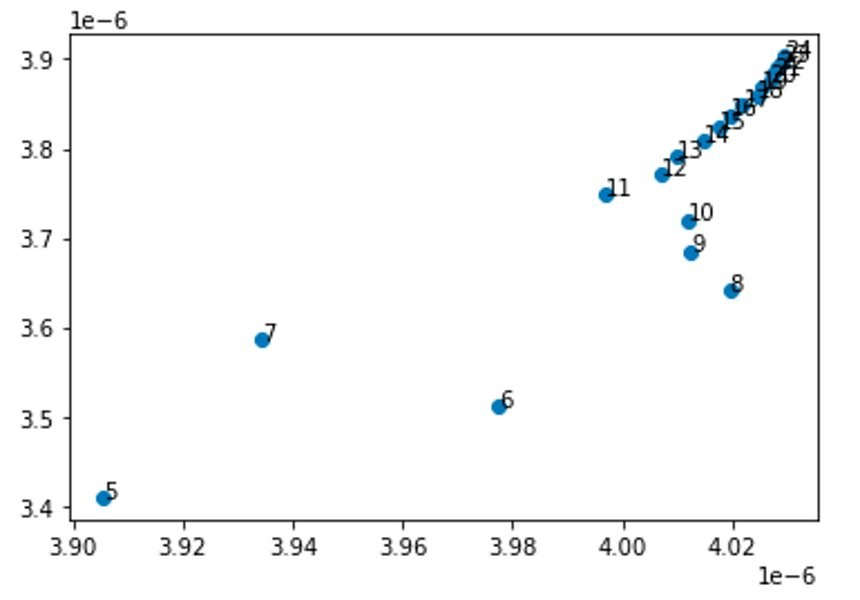
\includegraphics[width=\linewidth]{figures/svd_inter_intra.jpeg}
  \caption[Plot of inter-variance vs intra-variance]{Inter-variance (x-axis) vs intra-variance (y-axis) for SVD. The optimal number of dimensions comes out to be 6.}
  \label{fig:svd}
\end{figure}



\subsection{Finding optimal number of clusters}

We plotted an elbow graph for Within-Cluster Sum of Square (WCSS) \cite{bagirov2008modified} vs number of clusters to determine the optimal number of clusters for our clustering. WCSS is the sum of the squared distances between each point in a cluster and its centroid. As the number of cluster increases, the WCSS value decreases, giving us an elbow point where the WCSS value declines the most.  

The normalization of preference categories at a global level was not helping the model generalize, it was not calibrating the model for different user groups. We therefore incorporated the price of the device into the preference category vector, by normalizing the multi-hot category vector for each price bucket. Our reasoning here was that people buying devices in certain ranges would tend to have similar tastes. So, the preference categories vector now indicated how different the preferred categories were for a particular user as compared to other users in the same price bucket of the device.  

This helped us greatly in tuning the model. After all the iterations, the optimal number of clusters came out to be 6, as evidenced by the faint elbow in Figure \ref{fig:elbow}.

\begin{figure}
  \centering
  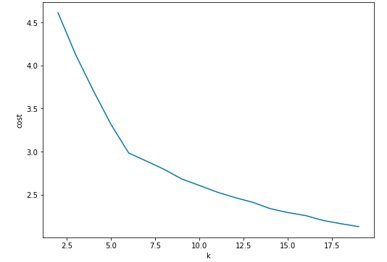
\includegraphics[width=\linewidth]{figures/elbow.jpeg}
  \caption[Elbow curve to identify optimum cluster number]{Plot of the elbow curve, WCSS vs number of clusters. The optimal number of clusters comes out to be 6.}
  \label{fig:elbow}
\end{figure}

On checking the feature distributions of the clusters, we were able to see clear distinctions, which meant that we had meaningful clusters. The distinction was clear enough to engineer user personas out of it, reproduced in Table \ref{tab:persona}.

\begin{table*}
  \caption{User personas emerging out of the clusters}
  \label{tab:persona}
  \begin{tabular}{llllll}
    \toprule
    Cluster&DPI&Tier&Gender&Price&Preference Categories (ordered by priority)\\
    \midrule
    0 & High & Mix & Male & Mix & Finance, Productivity, Entertainment\\
    1 & High & T1 \& T3 & Dominant Male & Mix & Shopping, Finance, Business, Social\\
    2 & High & Mix & Dominant Male & Middle & Finance, Social\\
    3 & Very Low & Mix & Mix & Low & Finance, Social, Entertainment\\
    4 & Low & Mix & Mix & Middle & Social, Entertainment, Finance, Shopping\\
    5 & Very High & Mix & Mix & High & Shopping, Finance, Entertainment, Productivity\\
  \bottomrule
\end{tabular}
\end{table*}



\subsection{Correlating with interaction data}

Our immediate next step was to check how well these clusters relate to the user’s interactions. More precisely, we wanted the users of these clusters to have different behaviors. For our dense users clustered in our training dataset, we looked at their interaction scores over a 30-day period. These interactions were calculated over a binary set of rewards, given when a user positively interacts with Bubbles. The scores were aggregated for the categories of the Bubbles interacted by the user, and then aggregated again at a cluster level. We thus prepared a weight matrix, which is the mapping between cluster numbers and mean interaction score of categories, for the users in those clusters. 

\begin{figure*}
  \centering
  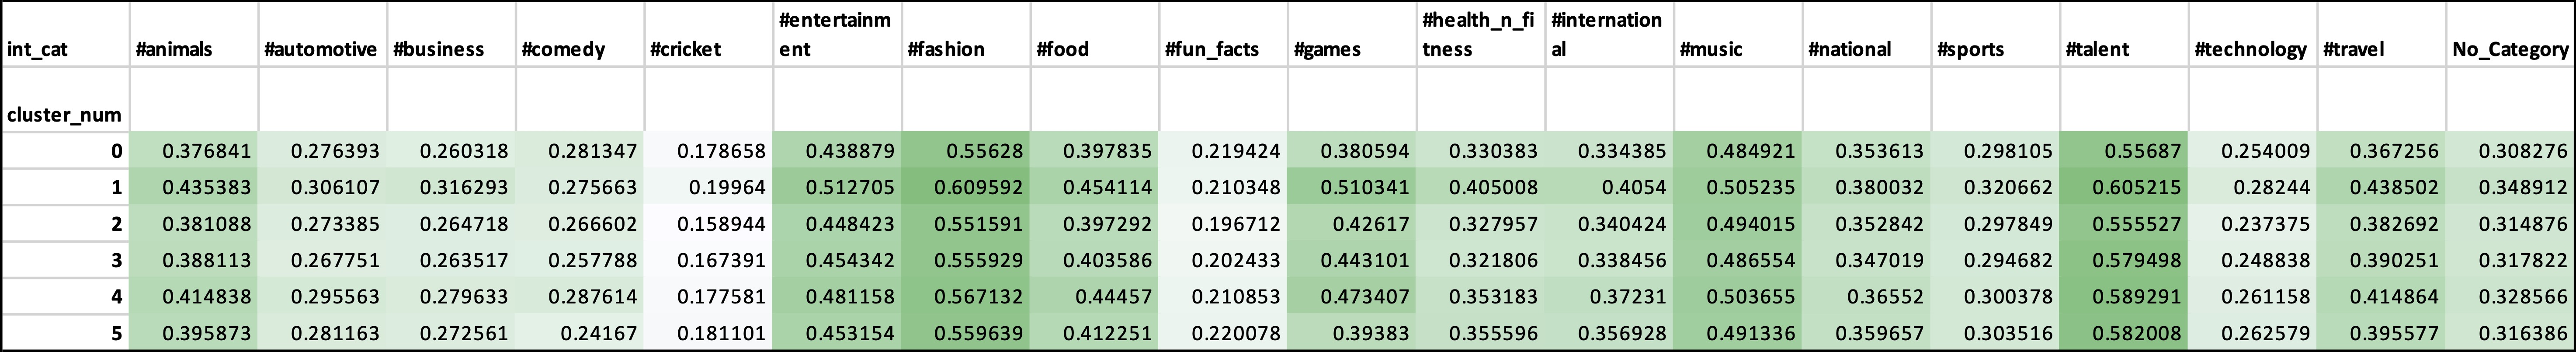
\includegraphics[width=\linewidth]{figures/mean_weight_matrix.jpg}
  \caption[Mean Weight Matrix]{A map of cluster number and the mean interaction score of the users belonging to the cluster}
  \label{fig:mean_weight_matrix}
\end{figure*}

Figure \ref{fig:mean_weight_matrix} represents this mean weight matrix. Here, the vertical bands mean that all the clusters behave generally similarly across the interaction categories. The very slight horizontal banding means there is a variation in the interaction behavior. But that was too slight a variation to have any predictive power.  

\begin{figure*}
  \centering
  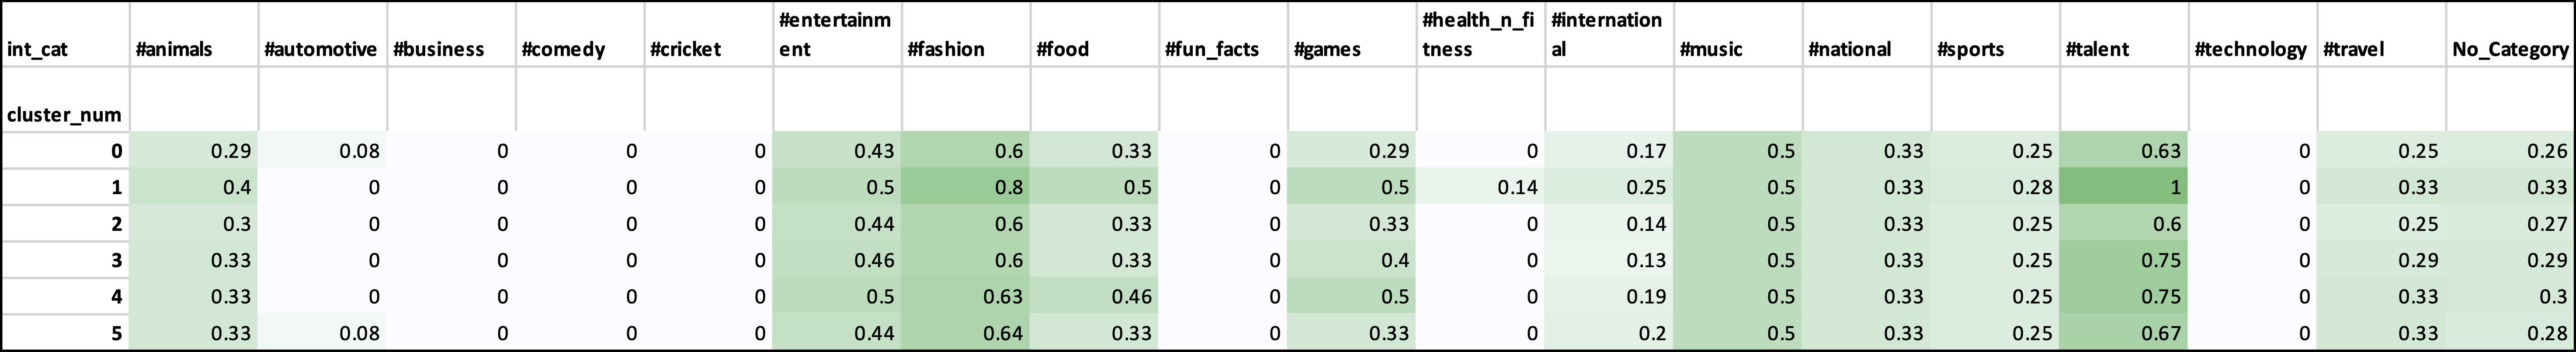
\includegraphics[width=\linewidth]{figures/median_weight_matrix.jpg}
  \caption[Median Weight Matrix]{A map of cluster number and the median interaction score of the users belonging to the cluster}
  \label{fig:median_weight_matrix}
\end{figure*}

Since mean interaction scores were possibly skewed due to outliers, we repeated the same exercise with median interaction scores and now the horizontal banding became more distinct, as shown in Figure \ref{fig:median_weight_matrix}. Notice how cluster 1 and 4 stand out generally in all categories, 0 and 5 in automotive, and cluster 1 in health and fitness. This highlighted a correlation between the clusters and the interaction categories that could be leveraged for sparse users’ recommendation.


\section{Implementation}

\subsection{The end-to-end solution}

The lookalike model works on the hypothesis that sparse users belonging to the same cluster as predicted by our k-means model (trained on dense users) should exhibit similar interaction preferences. By taking this preference into consideration in our ranking, we should notice a better reward rate and higher engagement from our sparse users – eventually turning them into dense users. 

Our recommendation system would therefore consist of: 

\begin{itemize}
    \item Identifying the cluster number that a cold or sparse user belongs to 
    \item Fetching the associated weight vector for the categories of the content 
    \item Ranking the Bubbles by using this vector as the defining rubric 
\end{itemize}

For the sake of our experiment, we will test this A/B on a set of 400,000 active users. The architecture overview is provided in figure \ref{fig:arch}.

\begin{figure*}
  \centering
  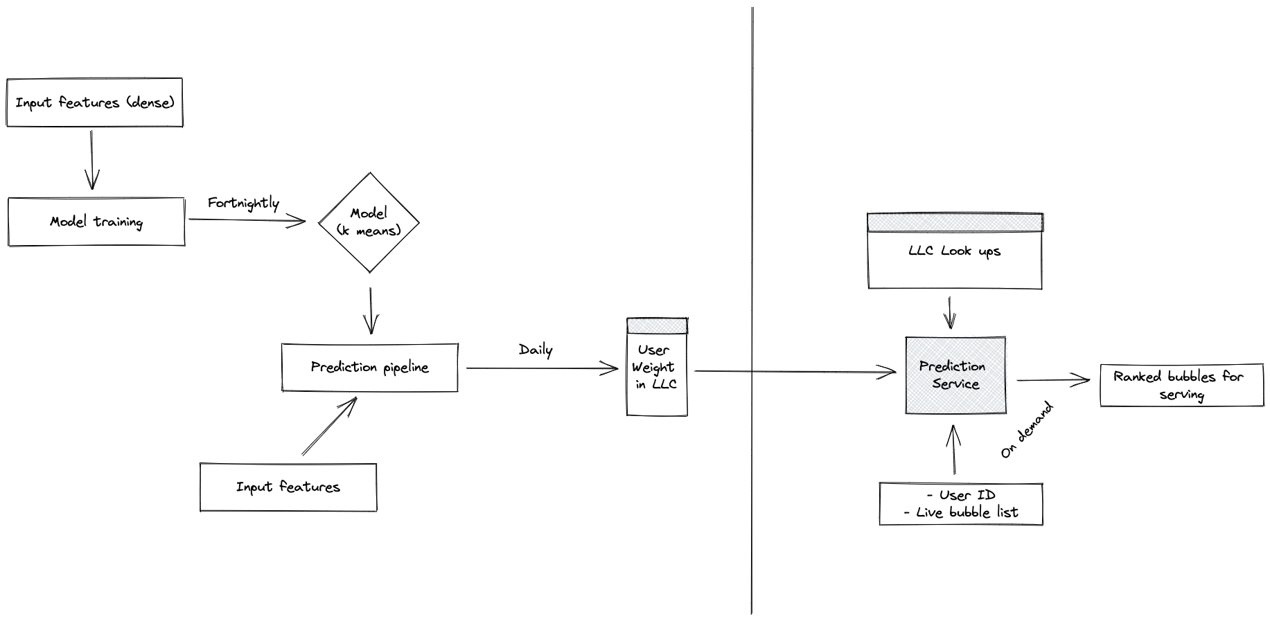
\includegraphics[width=\textwidth]{figures/arch.jpeg}
  \caption[Architecture diagram of the end-to-end system]{Overview of the end-to-end system design}
  \label{fig:arch}
\end{figure*}

\subsection{Specification of the prediction service}

Our recommendation systems at Glance operate under some tight constraints: 

\begin{itemize}
    \item Latency of the prediction model should be less than 150ms 
    \item The number of Bubbles ranked per user request can go up to 400 Bubbles per request 
    \item At any given time, we have roughly 4000 content pieces in our repository to be served, as they keep getting refreshed. 
\end{itemize}

We have one pipeline to train our clustering model on our dense users. We do not expect a lot of drift in the data, so this model could be refreshed as lazily as every fortnight. The users belong to our control subset, so that other model biases are not introduced into the dataset. This subset forms 10\% of our active user base, which has a very simple serving algorithm which we will compare ourselves with, called {\itshape Pacing}. 

A second pipeline runs at a daily cadence, to identify the cluster number of the users in our experiment. This pipeline loads the k-means model and runs clustering on target set of users. It then uses the weight matrix to identify the corresponding category weights for the user. The {\verb|[user_id, category_weight]|} mapping is saved in a low latency cache. This pipeline takes about 7 minutes to run. 

Our prediction service takes three inputs:  
\begin{itemize}
    \item {\verb|user_id|}: a unique identifier for the user in our system  
    \item {\verb|bubble_count|}: number of Bubbles to be ranked 
    \item and {\verb|live_bubbles|}: a candidate list of Bubbles to rank 
\end{itemize}

It fetches the {\verb|category_weight|} of the user from the low latency cache. It then looks up two attributes for every Bubble in {\verb|live_bubbles|}: category and global popularity of the Bubble. The global popularity of a Bubble is sampled from a beta distribution composed of the positive and negative interactions of the users on that Bubble, over a period of the previous 30 days. All the lookups are locally cached to avoid repeated network calls. 

The {\verb|category_weight|} of a user identifies a category affinity. We need to translate this to a Bubble level score. To do that we envision {\verb|bubble_count|} number of slots to fill with {\verb|live_bubbles|}. The {\verb|category_weight|} tells us which category the user is more likely to interact with. Multinomial sampling with the different categories weighed differently lets us divide bubble count into category slots. A category slot is filled in with the most popular bubble in the live bubbles list, according to global popularity score. 

The category weight only tells how likely a cluster is to interact with the categories and should not be interpreted as order of interaction. Say “fashion” had 0.5 and “sports” had 0.3 as their category weights for a certain cluster. This doesn't mean fashion content should come "first" while ranking the content, all this means is that fashion was preferred more as a category. Therefore, we do not encode the category weight into the final score associated with the Bubble and use it only to dictate the number of Bubbles. The popularity score serves as the final step to attach a score to every bubble. 

Two further tweaks make this ready for production: 
\begin{itemize}
    \item A 20\% reservation to explore categories uniformly, to better identify category affinity
    \begin{itemize}
        \item Essentially our model operates on 80\% of {\verb|bubble_count|}, with 20\% of the {\verb|bubble_count|} sampled from a uniform distribution of category weights 
    \end{itemize}
    \item A fallback mechanism for when {\verb|category_weight|} is unavailable for a user
    \begin{itemize}
        \item Because the pipeline runs at a daily cadence there would be users who would not be touched by the pipeline yet, and hence have no {\verb|category_weight|}. For such users we fallback to scoring the bubbles basis their global popularity, sampling from the global interaction distribution. 
    \end{itemize}
\end{itemize}

Because the final prediction service does only light weight calculations it is extremely fast. It can maintain a steady state p99 latency of 60ms. 

\begin{figure}[h]
  \centering
  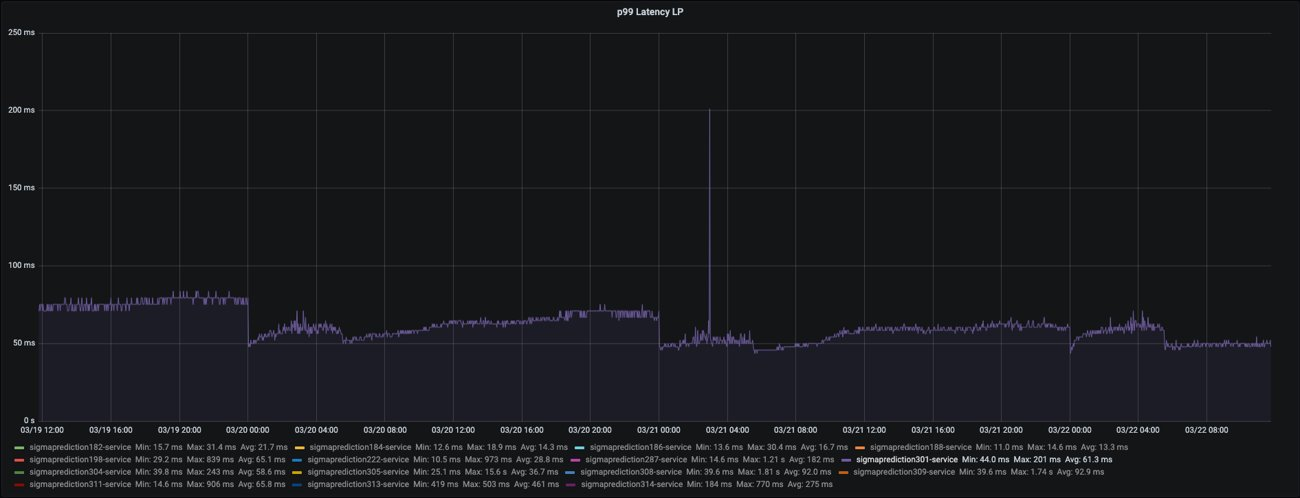
\includegraphics[width=\linewidth]{figures/latency.jpeg}
  \caption[P99 Latency of the prediction service]{Grafana dashboard showing the p99 latency of the prediction service, at a steady state of around 60ms}
  \label{fig:latency}
\end{figure}


\section{Results}

Our primary model of comparison is called Pacing. It is a simple rule-based model that “paces” or limits the Bubbles served to the user based on certain rules, and acts as the default baseline to compare performance against at Glance. We also benchmark our model, called {\verb|explorelookalikev1|}, against some of the other models active during that period. These include a user level Logistic Regression model ({\verb|userlrmodel1dot1|}) and a basic version of a Multi Armed Bandits model ({\verb|basemodelhighlights|}). We will look at the performance both at an overall level and at a cohort level; specifically at cold users. 

To measure engagement, we have two metrics: 
\begin{itemize}
    \item {\verb|Time Spent|}: Average duration a user spends on Glance in seconds, per day
    \item {\verb|Reward Rate|}: Average reward rate of the model, per day. Either at a Bubble or Glance level.
\end{itemize}

For the sake of confidentiality, the actual values of Time Spent have been masked. Reward Rate is a score calculated over an aggregation of positive interactions. These include such aspects as dwell time, explicit positive signals and virality.  

{\verb|explorelookalikev1|} consistently performs better than pacing across both the metrics, as seen in Figure \ref{fig:comp_pacing_overall}. On average it gets a 11.68\% delta over Pacing. The Reward Rate of our model is higher by 4.5\% on average.

\begin{figure}
    \centering
    \begin{subfigure}
      \centering
      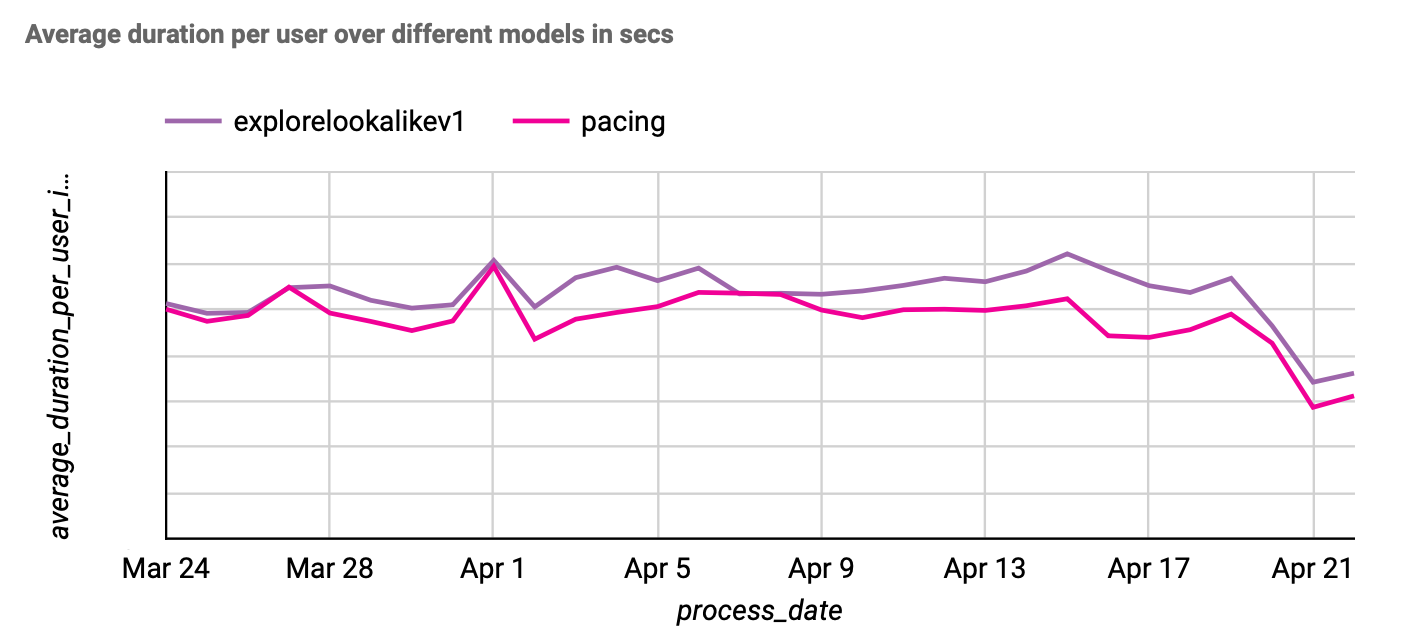
\includegraphics[width=\linewidth]{figures/DurationOverall-wrtPacing.png}
    \end{subfigure}%
    \begin{subfigure}
      \centering
      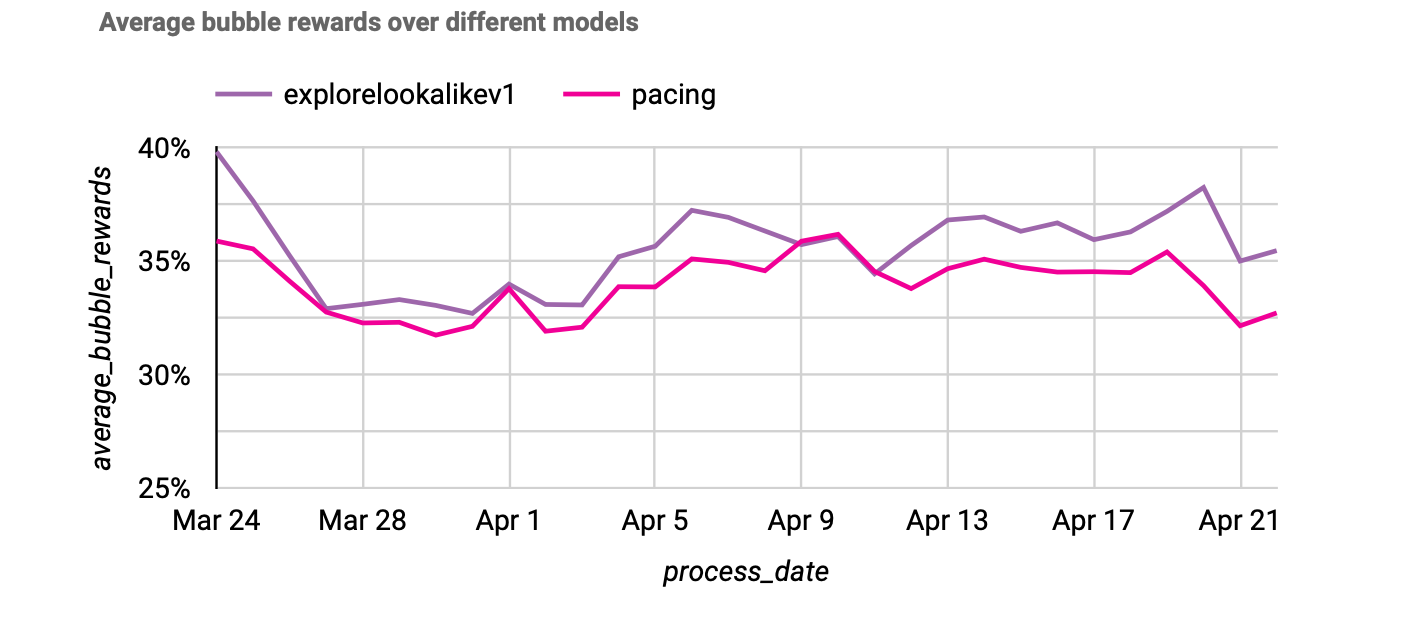
\includegraphics[width=\linewidth]{figures/BubRewardOverall-wrtPacing.png}
    \end{subfigure}
    \caption{Time spent (top) and Reward Rate (bottom) of our model as compared to Pacing, over all cohorts}
    \label{fig:comp_pacing_overall}
\end{figure}

When compared to the other models (Figure \ref{fig:comp_3_overall}) during the same period, our model routinely beats them on both the metrics, although by a smaller margin.  

\begin{figure}
    \centering
    \begin{subfigure}
      \centering
      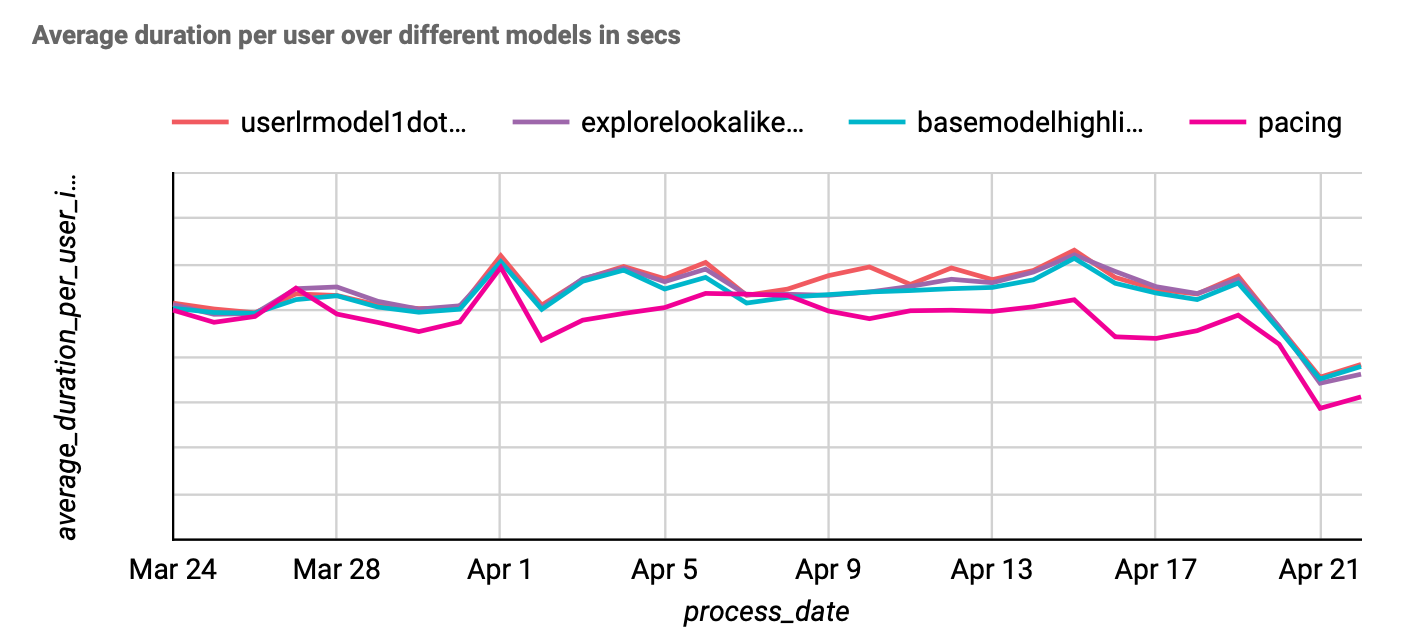
\includegraphics[width=\linewidth]{figures/DurationOverall-wrt3.png}
    \end{subfigure}%
    \begin{subfigure}
      \centering
      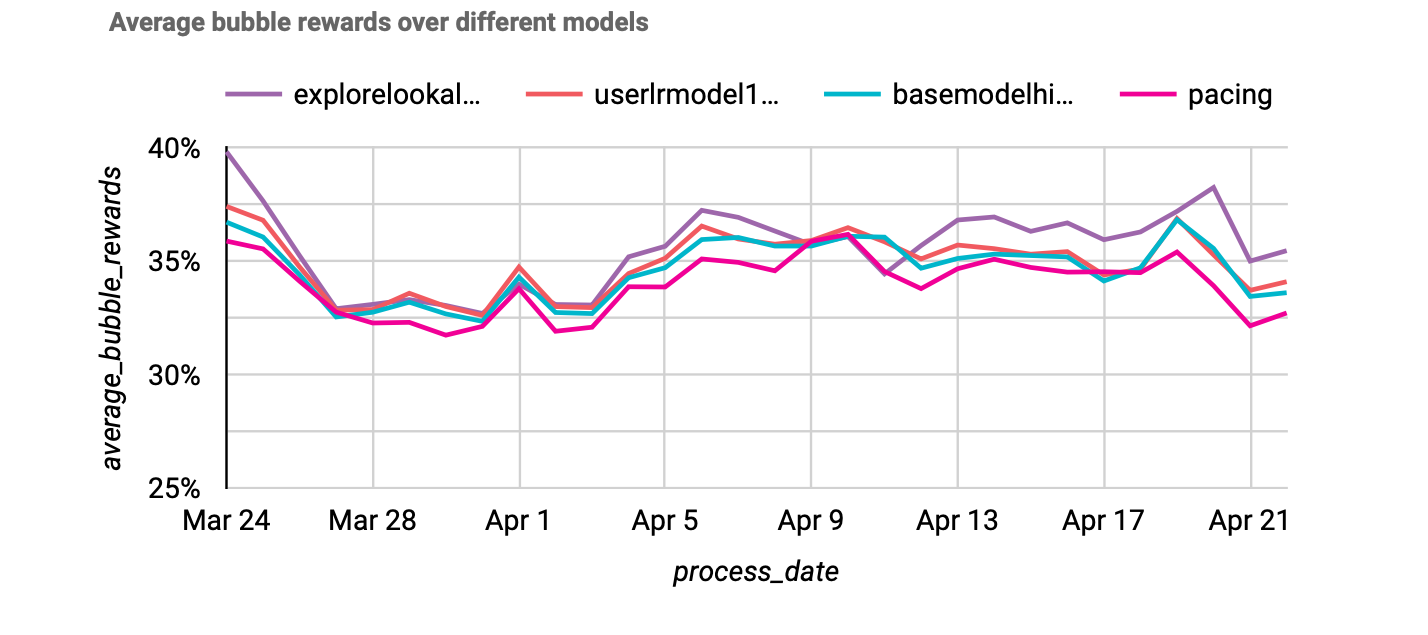
\includegraphics[width=\linewidth]{figures/BubRewardOverall-wrt3.png}
    \end{subfigure}
    \caption{Time spent (top) and Reward Rate (bottom) of our model as compared to other models, over all cohorts}
    \label{fig:comp_3_overall}
\end{figure}

Note that this across all the cohorts – cold, sparse, and dense. Because our model was trained on Dense users it was bound to perform well for them. It will not be sustainable, however, as at this stage it is only identifying popular content in specific categories for the users. If scaled it will not be able to explore content as well as a standard MAB. 

For Cold users (Figure \ref{fig:comp_pacing_cold}), the model performance comes out more distinctly. An average lift of 18.38\% in Time Spent and 5.76\% in Reward Rate as compared to Pacing. We also see competitive (and, at worst, at par) performance with respect to the other models (Figure \ref{fig:comp_3_cold}). 

\begin{figure}
    \centering
    \begin{subfigure}
      \centering
      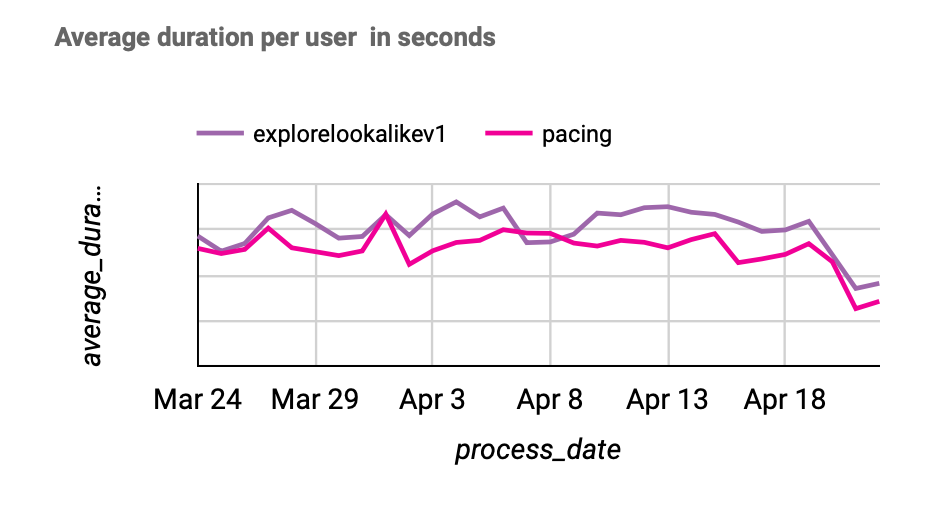
\includegraphics[width=\linewidth]{figures/DurationCold-wrtPacing.png}
    \end{subfigure}%
    \begin{subfigure}
      \centering
      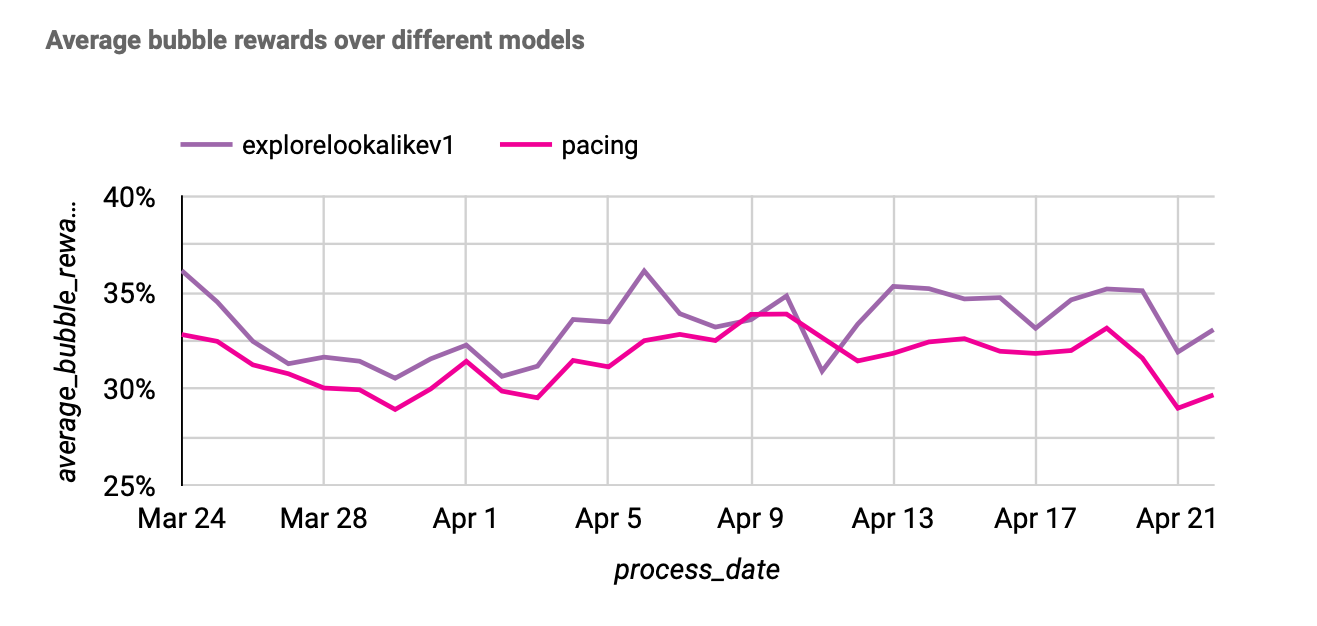
\includegraphics[width=\linewidth]{figures/BubRewardCold-wrtPacing.png}
    \end{subfigure}
    \caption{Time spent (top) and Reward Rate (bottom) of our model as compared to Pacing, for Cold Users}
    \label{fig:comp_pacing_cold}
\end{figure}

\begin{figure}
    \centering
    \begin{subfigure}
      \centering
      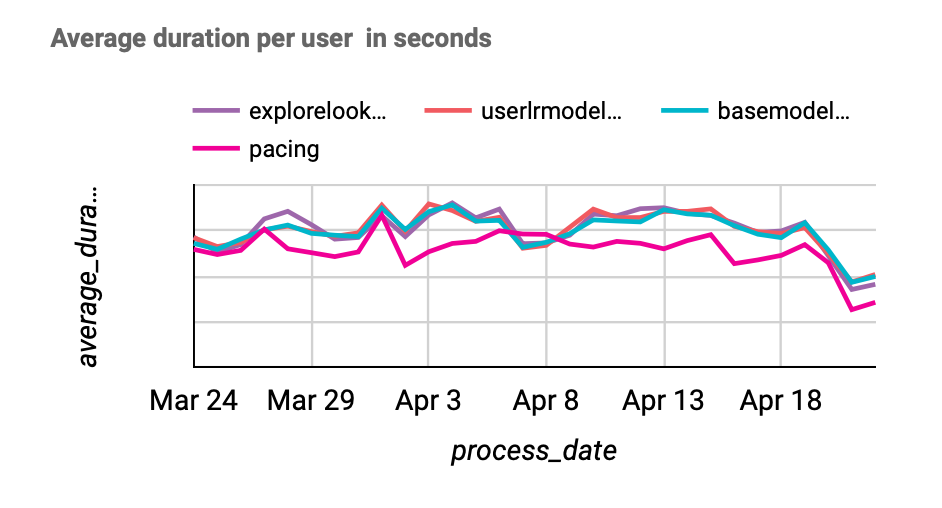
\includegraphics[width=\linewidth]{figures/DurationCold-wrt3.png}
    \end{subfigure}%
    \begin{subfigure}
      \centering
      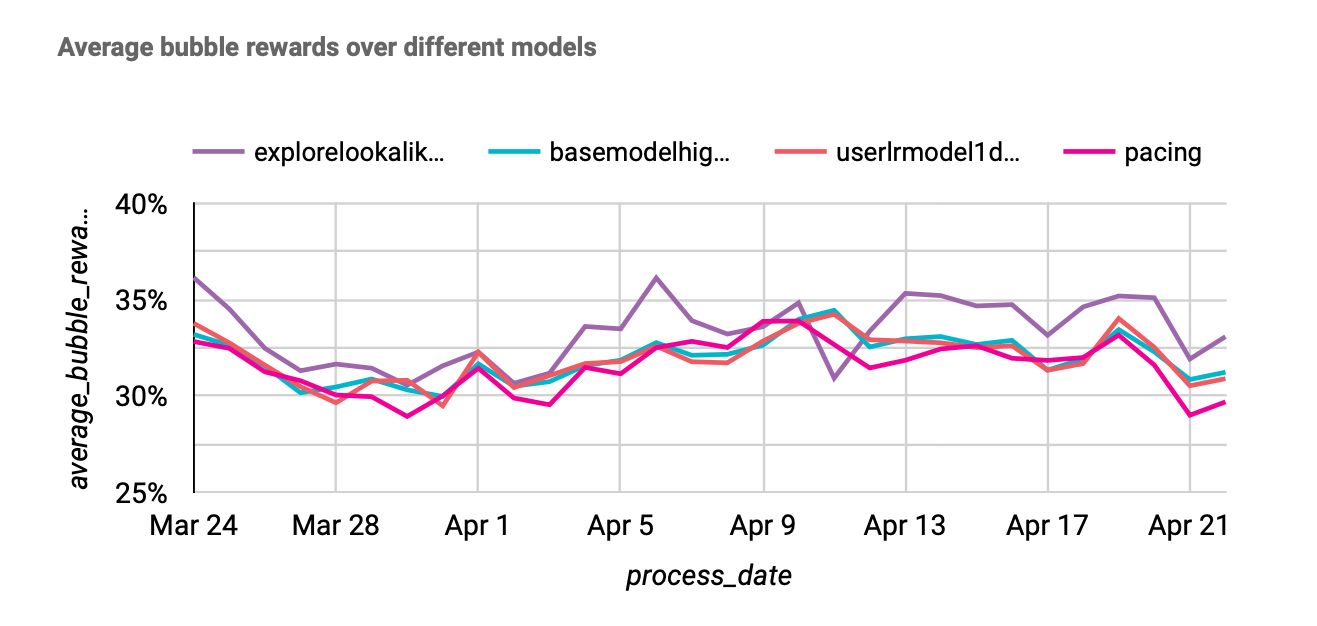
\includegraphics[width=\linewidth]{figures/BubRewardCold-wrt3.png}
    \end{subfigure}
    \caption{Time spent (top) and Reward Rate (bottom) of our model as compared to other models, for Cold Users}
    \label{fig:comp_3_cold}
\end{figure}

% \begin{figure*}
%     \centering
%     \begin{subfigure}
%       \centering
%       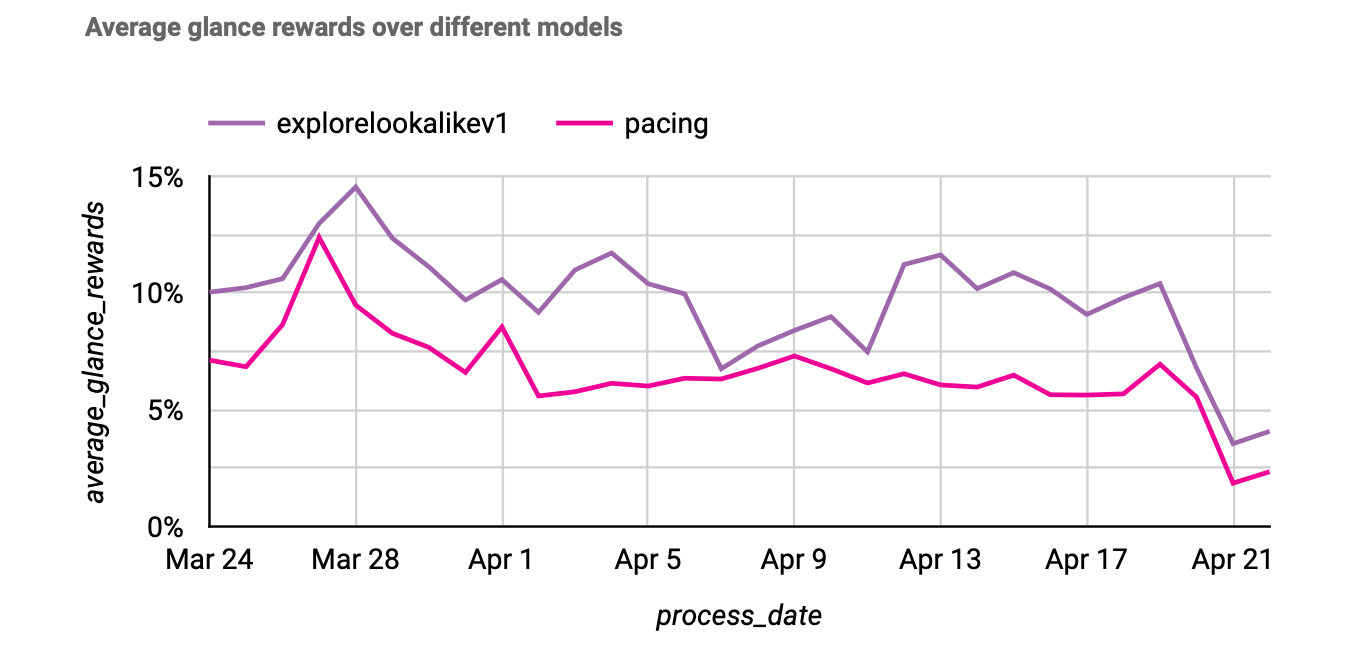
\includegraphics[width=0.45\textwidth]{figures/GlRewardCold-wrtPacing.png}
%     \end{subfigure}%
%     \begin{subfigure}
%       \centering
%       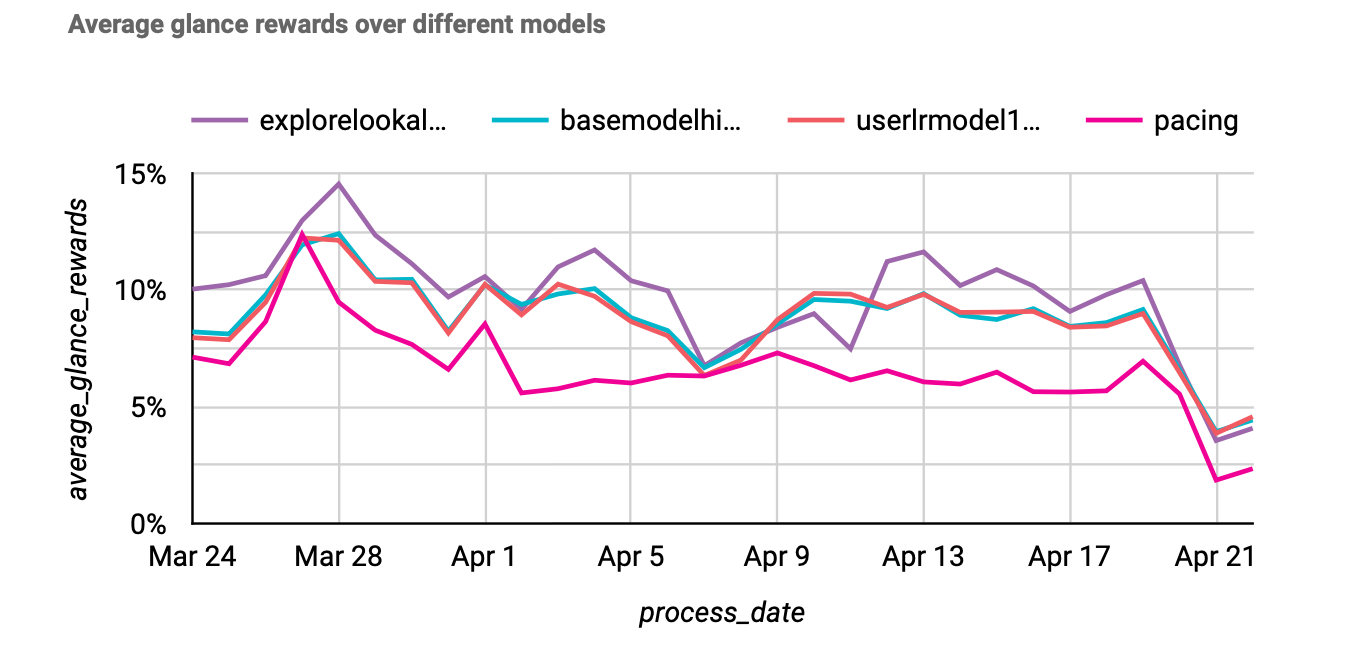
\includegraphics[width=0.45\textwidth]{figures/GlRewardCold-wrt3.png}
%     \end{subfigure}
%     \caption{Reward Rate at Glance level as compared to Pacing (left) and other models (right), for Cold Users}
%     \label{fig:comp_gl_reward}
% \end{figure*}

The improvement is especially stark when looked at the Reward Rate at Glance level, for Cold users (Figure \ref{fig:comp_gl_reward}. An average lift of 51.8\% as compared to Pacing and consistently beating out the other models. Our model, thus, performs well across all the metrics, especially so on Cold users.



\section{Conclusion and Future Work}

In this paper we showcased our clustering-based lookalike approach for recommending content to Cold and Sparse users. We show empirical evidence that the approach works, based on a real-world A/B experiment over a period of 30 days. 

For future iterations, the system is being modified to incorporate new, richer features to better define the clusters. Experiments are also underway to test other clustering methods like Spectral Clustering, which should bring out the latent representation of the clusters better. 
\newpage
\bibliographystyle{ACM-Reference-Format}
\bibliography{references}


% \section{Introduction}
% % The very first letter is a 2 line initial drop letter followed
% % by the rest of the first word in caps.
% % 
% % form to use if the first word consists of a single letter:
% % \IEEEPARstart{A}{demo} file is ....
% % 
% % form to use if you need the single drop letter followed by
% % normal text (unknown if ever used by the IEEE):
% % \IEEEPARstart{A}{}demo file is ....
% % 
% % Some journals put the first two words in caps:
% % \IEEEPARstart{T}{his demo} file is ....
% % 
% % Here we have the typical use of a "T" for an initial drop letter
% % and "HIS" in caps to complete the first word.
% \IEEEPARstart{T}{his} demo file is intended to serve as a ``starter file''
% for IEEE journal papers produced under \LaTeX\ using
% IEEEtran.cls version 1.8b and later.
% % You must have at least 2 lines in the paragraph with the drop letter
% % (should never be an issue)
% I wish you the best of success.

% \hfill mds
 
% \hfill August 26, 2015

% \subsection{Subsection Heading Here}
% Subsection text here.

% % needed in second column of first page if using \IEEEpubid
% %\IEEEpubidadjcol

% \subsubsection{Subsubsection Heading Here}
% Subsubsection text here.


% % An example of a floating figure using the graphicx package.
% % Note that \label must occur AFTER (or within) \caption.
% % For figures, \caption should occur after the \includegraphics.
% % Note that IEEEtran v1.7 and later has special internal code that
% % is designed to preserve the operation of \label within \caption
% % even when the captionsoff option is in effect. However, because
% % of issues like this, it may be the safest practice to put all your
% % \label just after \caption rather than within \caption{}.
% %
% % Reminder: the "draftcls" or "draftclsnofoot", not "draft", class
% % option should be used if it is desired that the figures are to be
% % displayed while in draft mode.
% %
% %\begin{figure}[!t]
% %\centering
% %\includegraphics[width=2.5in]{myfigure}
% % where an .eps filename suffix will be assumed under latex, 
% % and a .pdf suffix will be assumed for pdflatex; or what has been declared
% % via \DeclareGraphicsExtensions.
% %\caption{Simulation results for the network.}
% %\label{fig_sim}
% %\end{figure}

% % Note that the IEEE typically puts floats only at the top, even when this
% % results in a large percentage of a column being occupied by floats.


% % An example of a double column floating figure using two subfigures.
% % (The subfig.sty package must be loaded for this to work.)
% % The subfigure \label commands are set within each subfloat command,
% % and the \label for the overall figure must come after \caption.
% % \hfil is used as a separator to get equal spacing.
% % Watch out that the combined width of all the subfigures on a 
% % line do not exceed the text width or a line break will occur.
% %
% %\begin{figure*}[!t]
% %\centering
% %\subfloat[Case I]{\includegraphics[width=2.5in]{box}%
% %\label{fig_first_case}}
% %\hfil
% %\subfloat[Case II]{\includegraphics[width=2.5in]{box}%
% %\label{fig_second_case}}
% %\caption{Simulation results for the network.}
% %\label{fig_sim}
% %\end{figure*}
% %
% % Note that often IEEE papers with subfigures do not employ subfigure
% % captions (using the optional argument to \subfloat[]), but instead will
% % reference/describe all of them (a), (b), etc., within the main caption.
% % Be aware that for subfig.sty to generate the (a), (b), etc., subfigure
% % labels, the optional argument to \subfloat must be present. If a
% % subcaption is not desired, just leave its contents blank,
% % e.g., \subfloat[].


% % An example of a floating table. Note that, for IEEE style tables, the
% % \caption command should come BEFORE the table and, given that table
% % captions serve much like titles, are usually capitalized except for words
% % such as a, an, and, as, at, but, by, for, in, nor, of, on, or, the, to
% % and up, which are usually not capitalized unless they are the first or
% % last word of the caption. Table text will default to \footnotesize as
% % the IEEE normally uses this smaller font for tables.
% % The \label must come after \caption as always.
% %
% %\begin{table}[!t]
% %% increase table row spacing, adjust to taste
% %\renewcommand{\arraystretch}{1.3}
% % if using array.sty, it might be a good idea to tweak the value of
% % \extrarowheight as needed to properly center the text within the cells
% %\caption{An Example of a Table}
% %\label{table_example}
% %\centering
% %% Some packages, such as MDW tools, offer better commands for making tables
% %% than the plain LaTeX2e tabular which is used here.
% %\begin{tabular}{|c||c|}
% %\hline
% %One & Two\\
% %\hline
% %Three & Four\\
% %\hline
% %\end{tabular}
% %\end{table}


% % Note that the IEEE does not put floats in the very first column
% % - or typically anywhere on the first page for that matter. Also,
% % in-text middle ("here") positioning is typically not used, but it
% % is allowed and encouraged for Computer Society conferences (but
% % not Computer Society journals). Most IEEE journals/conferences use
% % top floats exclusively. 
% % Note that, LaTeX2e, unlike IEEE journals/conferences, places
% % footnotes above bottom floats. This can be corrected via the
% % \fnbelowfloat command of the stfloats package.




% \section{Conclusion}
% The conclusion goes here.





% % if have a single appendix:
% %\appendix[Proof of the Zonklar Equations]
% % or
% %\appendix  % for no appendix heading
% % do not use \section anymore after \appendix, only \section*
% % is possibly needed

% % use appendices with more than one appendix
% % then use \section to start each appendix
% % you must declare a \section before using any
% % \subsection or using \label (\appendices by itself
% % starts a section numbered zero.)
% %


% \appendices
% \section{Proof of the First Zonklar Equation}
% Appendix one text goes here.

% % you can choose not to have a title for an appendix
% % if you want by leaving the argument blank
% \section{}
% Appendix two text goes here.


% % use section* for acknowledgment
% \section*{Acknowledgment}


% The authors would like to thank...


% % Can use something like this to put references on a page
% % by themselves when using endfloat and the captionsoff option.
% \ifCLASSOPTIONcaptionsoff
%   \newpage
% \fi



% % trigger a \newpage just before the given reference
% % number - used to balance the columns on the last page
% % adjust value as needed - may need to be readjusted if
% % the document is modified later
% %\IEEEtriggeratref{8}
% % The "triggered" command can be changed if desired:
% %\IEEEtriggercmd{\enlargethispage{-5in}}

% % references section

% % can use a bibliography generated by BibTeX as a .bbl file
% % BibTeX documentation can be easily obtained at:
% % http://mirror.ctan.org/biblio/bibtex/contrib/doc/
% % The IEEEtran BibTeX style support page is at:
% % http://www.michaelshell.org/tex/ieeetran/bibtex/
% %\bibliographystyle{IEEEtran}
% % argument is your BibTeX string definitions and bibliography database(s)
% %\bibliography{IEEEabrv,../bib/paper}
% %
% % <OR> manually copy in the resultant .bbl file
% % set second argument of \begin to the number of references
% % (used to reserve space for the reference number labels box)
% \begin{thebibliography}{1}

% \bibitem{IEEEhowto:kopka}
% H.~Kopka and P.~W. Daly, \emph{A Guide to \LaTeX}, 3rd~ed.\hskip 1em plus
%   0.5em minus 0.4em\relax Harlow, England: Addison-Wesley, 1999.

% \end{thebibliography}

% % biography section
% % 
% % If you have an EPS/PDF photo (graphicx package needed) extra braces are
% % needed around the contents of the optional argument to biography to prevent
% % the LaTeX parser from getting confused when it sees the complicated
% % \includegraphics command within an optional argument. (You could create
% % your own custom macro containing the \includegraphics command to make things
% % simpler here.)
% %\begin{IEEEbiography}[{\includegraphics[width=1in,height=1.25in,clip,keepaspectratio]{mshell}}]{Michael Shell}
% % or if you just want to reserve a space for a photo:

% \begin{IEEEbiography}{Michael Shell}
% Biography text here.
% \end{IEEEbiography}

% % if you will not have a photo at all:
% \begin{IEEEbiographynophoto}{John Doe}
% Biography text here.
% \end{IEEEbiographynophoto}

% % insert where needed to balance the two columns on the last page with
% % biographies
% %\newpage

% \begin{IEEEbiographynophoto}{Jane Doe}
% Biography text here.
% \end{IEEEbiographynophoto}

% % You can push biographies down or up by placing
% % a \vfill before or after them. The appropriate
% % use of \vfill depends on what kind of text is
% % on the last page and whether or not the columns
% % are being equalized.

% %\vfill

% % Can be used to pull up biographies so that the bottom of the last one
% % is flush with the other column.
% %\enlargethispage{-5in}



% % that's all folks
\end{document}


